
\chapter{The Standard Model of Particle Physics}

% http://en.wikipedia.org/wiki/History_of_science
%Humans have been trying to understand the world around us since the beginning of recorded history. In ancient civilizations, through observation and experimentation, information on astronomy, physiology, chemistry, and classification was learned and passed on through oral tradition and writing. With this information many diverse theories and models to the governing rules of the Universe were proposed. In order to judge these theories the experimental method was developed. With this framework facts were uncovered through experimentation to test if these theories were right or wrong. In various cultures across the world knowledge of the world grew and the explanatory theories grew more refined.

%Scientific knowledge grew in spurts and pockets until 1543 with the beginning of the Scientific Revolution. This period saw the work of many famous scientists like Nicolaus Copernicus, Galileo Galilei, Blaise Pascal, and more, until the publication of Isaac Newton's ``Mathematical Principles of Natural Philosophy" in 1687. The scientific method was further developed  emphasizing experimentation and reason to explain the world. With the foundation work of previous scientists, the 18th century ``Age of Enlightenment" broke upon Europe. Based firmly on the work of Newton, Pascal, and others the developments of modern mathematics, physics, and technology was accomplished.

%In particular interest to physics, Isaac Newton proposed two successful physical theories: the laws of motion and the law of gravitation. These theories laid the backbone for classical mechanics and the theory of gravity. Further in the 19th century scientists like Michael Faraday and Georg Ohm studied electricity and magnetism with the eventual unification of the two into Maxwell's equations, creating the theory of electromagnetism.  

%In 1960 Sheldon Glashow combined electromagnetism and weak interactions together to form the basis of the electroweak theory of interactions.\cite{Glashow1961} This allowed Steven Weinberg and Abdus Salam to incorporate the Higgs mechanism into Glashow's electroweak theory in 1967, giving it its modern form.

This Chapter will give an introduction to the current theoretical framework in elementary particle physics.  We will describe the Standard Model and the motivation behind the Higgs mechanism.

Natural units will be used, i.e. $\hbar$ = c = 1, in this analysis unless otherwise specified.
%\section{Introduction}	


\section{Particles and Forces}

The Standard Model describes matter as comprised of 3 families which each contain 4 elementary particles.  Each of these particles are spin 1/2 fermions. Fermions are particles that follow the Pauli exclusion.  This principle states that the wave function of identical fermions is anti-symmetric to the exchange of the two particles\cite{Griffiths:2004}.  The first family is the building blocks of all ordinary matter while the second and third families are heavy copies of the first.  The corresponding particles that belong in the various families are said to have different flavor.  There is a natural division of the fermions into two groups.  These are leptons and quarks, and their classification can be seen in Table~\ref{tab:threegenerations}.  Quarks are never found isolated in nature, but are constituents of composite particles called hadrons.  The most common examples of hadrons are protons (two up quarks and one down quark) and neutrons (one up quark and two down quarks).  There are over 100 different hadrons which have led particle physicists to refer to them and other particles collectively as the Particle Zoo.  In contrast to quarks, leptons are found in free states and are not constituents of compound particles.

Interactions between particles are mediated through the exchange of force carriers which are bosons.  Bosons are particles which have integer spin and do not obey the Pauli exclusion principle which means they can occupy the same quantum state as other identical bosons.  The force carrier bosons are summarized in Table~\ref{tab:FundamentalForces}.  Throughout this thesis, the gravitational interaction, which is mediated by the theorized graviton, will not be taken into account because at the mass and distance ranges studied the interactions are negligible. The W and Z bosons mediate the weak force which is responsible for both radioactive decay and nuclear fusion of subatomic particles. The term weak is used because the strength of the field is typically several magnitudes of order less than both the strong force and electromagnetism.  Also, because the masses of the W and Z bosons are so large, the weak force has a very short range, around $10^{-17} - 10^{-16}$m\cite{Christman:2001}.  The strong force is mediated by the gluons and is around 100 times stronger than electromagnetism while working at the atomic scale.  This force binds quarks together to form hadrons, and binds protons and neutrons together to form the nucleus of atoms. The electromagnetic force is mediated by the photon and works on an infinite scale but falls off proportional to the square of the distance.  

The Standard Model describes these interactions using two theories. Quantum Chromodynamics (QCD) describes the strong force while the theory of the electroweak interaction \cite{Glashow1961} unifies the electromagnetic and weak interactions as described earlier. The following section will describe in more detail the electroweak interaction because it is the primary decay of interest to this work.






%There are four forces that govern the universe. These are the gravitational, electromagnetic, weak, and strong forces. The gravitational force is the weakest force and is primarily important in the interactions of large bodies, but does not play a significant roll in the interactions of particles. Attractions between charged particles are provided by the electromagnetic force. This is the primary force responsible for building atoms and molecules. The weak force is the motivator of radioactivity and fusion, while the strong force binds quarks into nucleons and nucleons to nuclei.

%Our current understanding is that quarks and leptons are the the basic constituents of all matter. Leptons are spin 1/2 particles with a charge of -1. They do not participate in the strong interaction and additionally each one has a corresponding neutrino.  These leptons are the electron, muon, and tau.

%Quarks are the building blocks of hadrons and are held together by the strong force.  There are three generations of quarks and leptons which are listed in Table~\ref{tab:threegenerations}.


\begin{table}[htb]
\caption{%
  \small The three generations of spin $\dfrac{1}{2}$ particles. %
}
\begin{center}
\begin{tabular}{ c c c c c c c c }
charge       & -1     & -2/3 & -1/3 & 0 & +1/3 & +2/3 & +1\\ \hline
$1^{st}$ family & $\Pem$ & $\Paqu$ & $\Pqd$ & $\Pgne , \Pagne$ & $\Paqd$ & $\Pqu$ & $\Pep$\\
$2^{nd}$ family & $\Pgmm$ & $\Paqc$ & $\Pqs$ & $\Pgngm , \Pagngm$ & $\Paqs$ & $\Pqc$ & $\Pgmp$\\
$3^{rd}$ family & $\Pgtm$ & $\Paqt$ & $\Pqb$ & $\Pgngt , \Pagngt$ & $\Paqb$ & $\Pqt$ & $\Pgmp$\\
\end{tabular}
\end{center}
\label{tab:threegenerations}
\end{table}

\begin{center}
\begin{table}[htb]
\caption{%
  \small The four forces and their associated gauge bosons. Charge is in units of the proton charge.%
}
\begin{center}
\begin{tabular}{ c c c c }
Force  & Boson    & Charge & Mass \\ \hline
Gravitational & graviton(G) & 0 & ? \\
Electromagnetic & photon($\gamma$) & 0 & 0 \\

\multirow{2}{*}{Weak} & W boson($W^{\pm}$) & $\pm$1 & 81 GeV \\
                      & Z boson(Z) & 0 & 92 GeV \\

Strong & gluon(g) & 0      & 0 \\
\end{tabular}
\end{center}
\label{tab:FundamentalForces}
\end{table}

\end{center}




\section{The Electroweak Interaction}

Quantum Electrodynamics (QED) is a quantum field theory that describes the electromagnetic interaction. A problem in many field theories is that the amplitude of many processes needs to be calculated by integrating over all possible values of particle momentum and energy.  This creates logarithmic divergences in these integrals, which are nonphysical. A process called re-normalization solves this problem~\cite{Peskin:1995}.  Re-normalization involves separating the divergent parts and canceling out the non-physical parts.  Many fields are not renormalizable, but in the early 1970's Hooft, Veltman, and others showed that gauge theories can be re-normalized\cite{Hooft:1971}\cite{Hooft:1972}.

Gauge theories are theories that require their Lagrangian to be invariant under a group of local transformations. The possible invariant transformations, which are called gauge transformations, together form a Lie group.  The group of local invariance is called a gauge group and has a corresponding gauge field which is included in the Lagrangian to ensure invariance under local group transformations.  The quanta of gauge fields are gauge bosons\cite{Wiki:Guage_Theory}.  In this work a detailed derivation of the electroweak Lagrangian will not be provided, but will simply be summarized.

The theory of electromagnetic interaction is based on the gauge group $U(1)_{EM}$.  The quantum number in this theory that is conserved is the electric charge (Q).  Local invariance condition under the $U(1)_{EM}$ group leads to a massless vector boson which is the photon.  To combine both the electromagnetic and weak interaction, the gauge symmetry is extended to the group $ S U(2)_{I} \otimes U(1)_{Y}$.  The three components of $t^{a} = \dfrac{1}{2}\tau^{a}$ ($\tau^{a}$ are the Pauli matrices), where $t^{a}$ is the weak isospin operator, are the generators of the $S U(2)_{I}$ group.  The weak hypercharge $Y$ operator is the generator of the $ U(1)_{Y}$ group. Using $I_{3}$ as the third component of the weak isospin, these quantum numbers satisfy equation~\ref{eq:electroweak_quantum}.

\begin{equation} Q = I_{3} + \dfrac{Y}{2} \label{eq:electroweak_quantum}\end{equation}

In table~\ref{tab:QuantumNumbers} the quantum numbers of the fermions are given where $u = u,c,t$, $d = d,s,b$, $l = e,\mu,\tau$, and $\nu = \nu_{e}, \nu_{\mu}, \nu_{\tau}$.


\begin{center}
\begin{table}[htb]
\caption{%
  \small Electric charge (Q), isospin ($I_{3}$), and hypercharge ($Y$) of the fermions.
}
\begin{center}
\begin{tabular}{ c c c c }
\hline & Q & $I_{3}$ & $Y$ \\ \hline \hline
$u$   & $^2/_3$  & $^1/_2$  & $^1/_3$ \\
$d$   & $-^1/_3$ & $-^1/_2$ & $^1/_3$ \\ \hline \hline
$l$   & $-1$            & $-^1/_2$ & $-1$ \\
$\nu$ & $0$             & $^1/_2$  & $-1$ \\
\hline
\end{tabular}
\end{center}
\label{tab:QuantumNumbers}
\end{table}

\end{center}

Just like the requirement of local gauge invariance for the $U(1)_{EM}$ group gives a massless vector field, the group $ S U(2)_{I} \otimes U(1)_{Y}$ now has four massless vector fields.  These fields are $W^{1,2,3}_{\mu}$ and $B_{\mu}$.  These fields do not represent physical fields, but the physical fields are given by linear combinations of them.  The W bosons, $W^+$ and $W^-$, are described in equation~\ref{eq:Ws}, the Z boson in equation~\ref{eq:Z}, and the $\gamma$ boson in equation~\ref{eq:gamma}.

\begin{equation} W^{\pm}_{\mu} = \sqrt{\dfrac{1}{2}}(W^1_{\mu} \mp iW^2_{\mu}) \label{eq:Ws}\end{equation}
\begin{equation} Z_{\mu} = -B_{\mu} sin \theta_W + W^3_{\mu} cos \theta_W \label{eq:Z}\end{equation}
\begin{equation} A_{\mu} = B_{\mu} cos \theta_W + W^3_{\mu} sin \theta_W \label{eq:gamma}\end{equation}

The Weinberg angle ($\theta_W$) is an open parameter of the standard model and can be determined empirically using the relation in equation~\ref{eq:weinberg}, where $m_W$ and $m_Z$ are the respective masses of the W and Z bosons. 

\begin{equation} cos \theta_W = \dfrac{m_W}{m_Z} \label{eq:weinberg}\end{equation}









\section{The Higgs Boson}

The electroweak theory as described so far describes all particles as massless.  Introducing a mass term for the gauge bosons would violate gauge invariance which is essential for re-normalization.  To agree with experimental findings, some of the gauge bosons must have mass, as well as mass being needed to successfully describe the weak interaction phenomenology. By introducing the Higgs mechanism fermions and $W^{\pm}$, $Z$ bosons are allowed to have mass~\cite{Dawson98}.   Introducing a complex scalar $S U(2)$ doublet, $\Phi$ given in equation~\ref{eq:doublet}, allows the introduction of such a mechanism.

\begin{equation} \Phi = \left( \genfrac{}{}{0pt}{}{\phi^+}{\phi^0}  \right) \label{eq:doublet}\end{equation}

This field is introduced to the electroweak Lagrangian in the term ~\ref{eq:L_ewsb} \begin{equation} \mathcal{L}_{H}  = (D^{\mu}\Phi)^{\dagger}(D_{\mu}\Phi) + V(\Phi^{\dagger} \Phi), \label{eq:L_ewsb}\end{equation} where $D_{\mu}$ is the covariant derivative. The $\Phi$ field has the quantum numbers as seen in table~\ref{tab:phi_QuantumNumbers} and has a potential that can be written as in equation~\ref{eq:potential}.  This potential can be seen graphically in Figure~\ref{fig:higgs_potential}.

\begin{center}
\begin{table}[htb]
\caption{\small   Electric charge (Q), isospin ($I_{3}$), and hypercharge ($Y$) of the $\Phi$ field.
}
\begin{center}
\begin{tabular}{ c c c c }
\hline     & Q    & $I_{3}$ & $Y$ \\ \hline \hline
$\phi^+$   & $1$  & $^1/_2$  & $1$ \\
$\phi^0$   & $0$  & $-^1/_2$ & $1$ \\ \hline
\hline
\end{tabular}
\end{center}
\label{tab:phi_QuantumNumbers}
\end{table}

\end{center}

\begin{equation} V(\Phi^{\dagger} \Phi) = -\mu^2 \Phi^{\dagger} \Phi - \lambda (\Phi^{\dagger} \Phi)^2 \label{eq:potential}\end{equation}

When $\mu^2 < 0$ and $\lambda > 0$, we get the minimum to be at $\dfrac{\nu^2}{2}$, where $\nu^2 = -\dfrac{-\mu^2}{\lambda}$ as seen in equation~\ref{eq:minimum}.  The minimum of this potential does not correspond to a single value of $\Phi$ and these values are non-zero. The lowest energy state is arbitrary and is not invariant under rotations.  This loss of rotational invariance is referred to as spontaneous symmetry breaking.  
\begin{equation} \Phi^{\dagger} \Phi = \dfrac{1}{2} ( \Phi^2_1 + \Phi^2_2 + \Phi^2_3 + \Phi^2_4) = -\dfrac{\mu^2}{2\lambda} \equiv \dfrac{\nu^2}{2} \label{eq:minimum}\end{equation}

The spontaneous symmetry breaking introduces mass terms for the $W^{\pm}$ and $Z$ fields as well as a scalar field, which is the Higgs field.  The Higgs field also gains mass itself.  Spontaneously breaking a symmetry does not eliminate the symmetry but hides it under the choice of the ground state.  Furthermore, the Higgs field is invariant under the $U(1)_{EM}$ group, leaving electromagnetic symmetry unbroken. The photon remains massless because it does not couple to the Higgs boson.

\begin{figure}[htb]
\centering
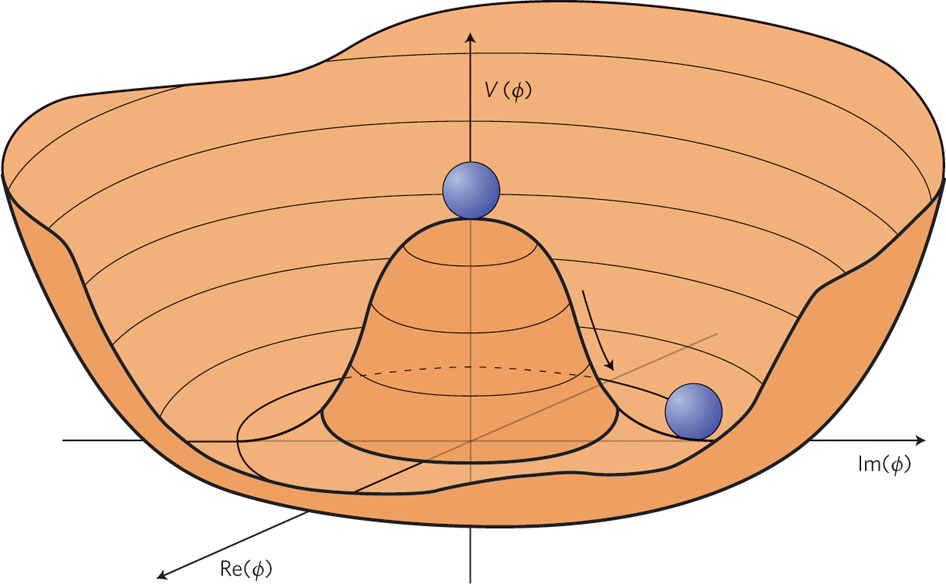
\includegraphics[width=0.9\textwidth]{StandardModel/higgs_potential.jpg}
\caption{\small An effective potential, V($\Phi$), that leads to spontaneous symmetry breaking.~\cite{Eyeonaprize2011} }
\label{fig:higgs_potential}
\end{figure}



\subsection{Higgs Boson Mass}

The Higgs boson mass is the only one of the 18 free parameters of the Standard Model~\cite{Englert1964} that was still undetermined at the start up of the LHC. While the mass of the Higgs boson is dependent on the parameters $\nu$ and $\lambda$, only $\nu$ can be estimated from another parameter.  Despite theoretically not being able to determine the Higgs boson mass, there are both theoretical and experimental constraints on the Higgs mass.  These come from both direct and indirect searches at various colliders.


\subsubsection{Theoretical Constraints}


The scalar potential needs to be bounded from below, even after including radiative corrections.  This gives a lower bound on $m_H$ as well.  If the quartic coupling $\lambda(\mu)$ stays positive then this requirement is fulfilled.  This is true at least until $\mu\sim\Lambda$ which is the maximum energy scale wherein the theory is still applicable~\cite{Ridolfi2001}. The relation $m_H^2\simeq 2\lambda(m_Z)v^2$ defines a $\Lambda$-dependent lower bound on $m_H$. This shows that for smaller values of $\lambda(m_Z)$ the $\Lambda$ scale also becomes smaller.  This leads to $\lambda$ becoming negative which means the scalar potential is no longer bounded.  The absolute minimum or vacuum stability is shown by the dashed line in figure~\ref{fig:bothbounds}. If the vacuum stability is only a local constraint we get a slightly looser lower bound as shown in the dot-dashed line in figure~\ref{fig:bothbounds}.


\begin{figure}[htb]
\centering
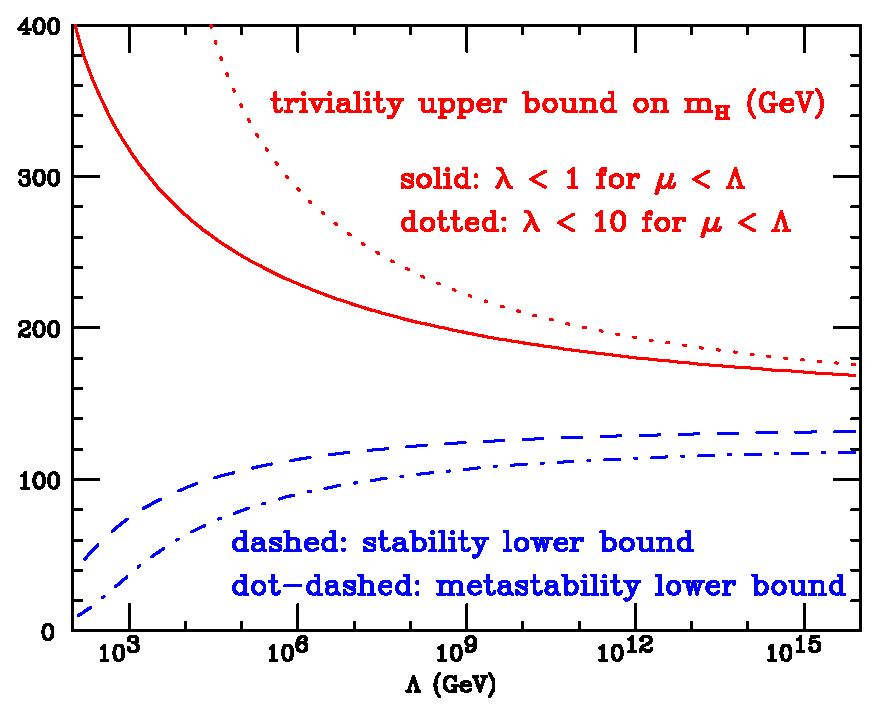
\includegraphics[width=0.9\textwidth]{StandardModel/bothbounds.eps}
\caption{Upper and lower bounds on the Higgs mass.~\cite{Ridolfi2001} }
\label{fig:bothbounds}
\end{figure}

% from the paper
%The smaller is $\lambda(m_Z)$, the smaller becomes the scale $\Lambda$ at which $\lambda$ becomes negative and the scalar potential unbounded. 
%Since $m_H^2\simeq 2\lambda(m_Z)v^2$, this implies a $\Lambda$-dependent lower bound on $m_H$.


The unitarity of the scattering matrix gives an upper bound on the Higgs mass.  This can be seen in the electric scattering of $Z$ bosons, $Z Z \to Z Z$.  In the limit that $s\gg m_Z^2$ we have:
\begin{equation} {\cal M}=-\frac{m_H^2}{v^2}\left[\frac{s}{s-m_H^2}+\frac{t}{t-m_H^2}+\frac{u}{u-m_H^2}\right] \label{eq:unitarity1}\end{equation}

Now with $J=0$ then the amplitude of ${\cal M}$ gives us:
\begin{equation}|{\cal M}_0|^2\to\left[\frac{3}{16\pi}\frac{m_H^2}{v^2}\right]^2<\frac{s}{s-4m_Z^2}\label{eq:unitarity2}\end{equation}

Since we said that $s\gg m_Z^2$ we get that $m_H<\sqrt{\frac{16\pi}{3}}\,v\sim 1\;{\rm TeV}$. Similarly if we look at $Z W \to Z W$ then the limit is $\sim 800$~GeV. There is another more restrictive constraint that is called the triviality bound. This is found by requiring that $\lambda$ is finite all the way to the $\Lambda$ scale.  When these limits are taken to the grand unification scale or Plank scale ($\Lambda ~ 10^{19}$GeV) there is an extreme upper bound of 180 GeV~\cite{Ridolfi2001}.  Together with the extreme limits of the lower bound shows a Higgs mass should be in the range  of somewhere 130 GeV to 180 GeV as seen in Figure~\ref{fig:bothbounds}.  While this is a bit extreme, it does make sense for colliders to search up to a range of 1 TeV while focusing on the lower ranges.

\subsubsection{Experimental Constraints before the LHC}

In addition to the theoretical bounds, there were both direct and indirect measurements on the Higgs mass. Direct searches for the Higgs have mostly come from the Large Electron-Positron Collider (LEP) at Cern and the Tevatron at Fermilab~\cite{ALEPH:2010aa}. This search has been a driving force in high-energy experiments for the last several decades.  A brief overview of the constraints will be given below.
 Direct searches using data from LEP excluded the $m_H$ below 114.4 GeV at a 95\% C.L. ~\cite{Barate:2003sz}. LEP was an $e^+e^-$ accelerator that ran from 1989 to 2000. The main production mechanism at LEP was $e^+e^- \rightarrow Z^* \rightarrow ZH$ where a Higgs is radiated by a virtual Z boson.  This process is often referred to as ``Higgs-strahlung''.  The results can be seen in figure~\ref{fig:adlocls}.

\begin{figure}[htb]
\centering
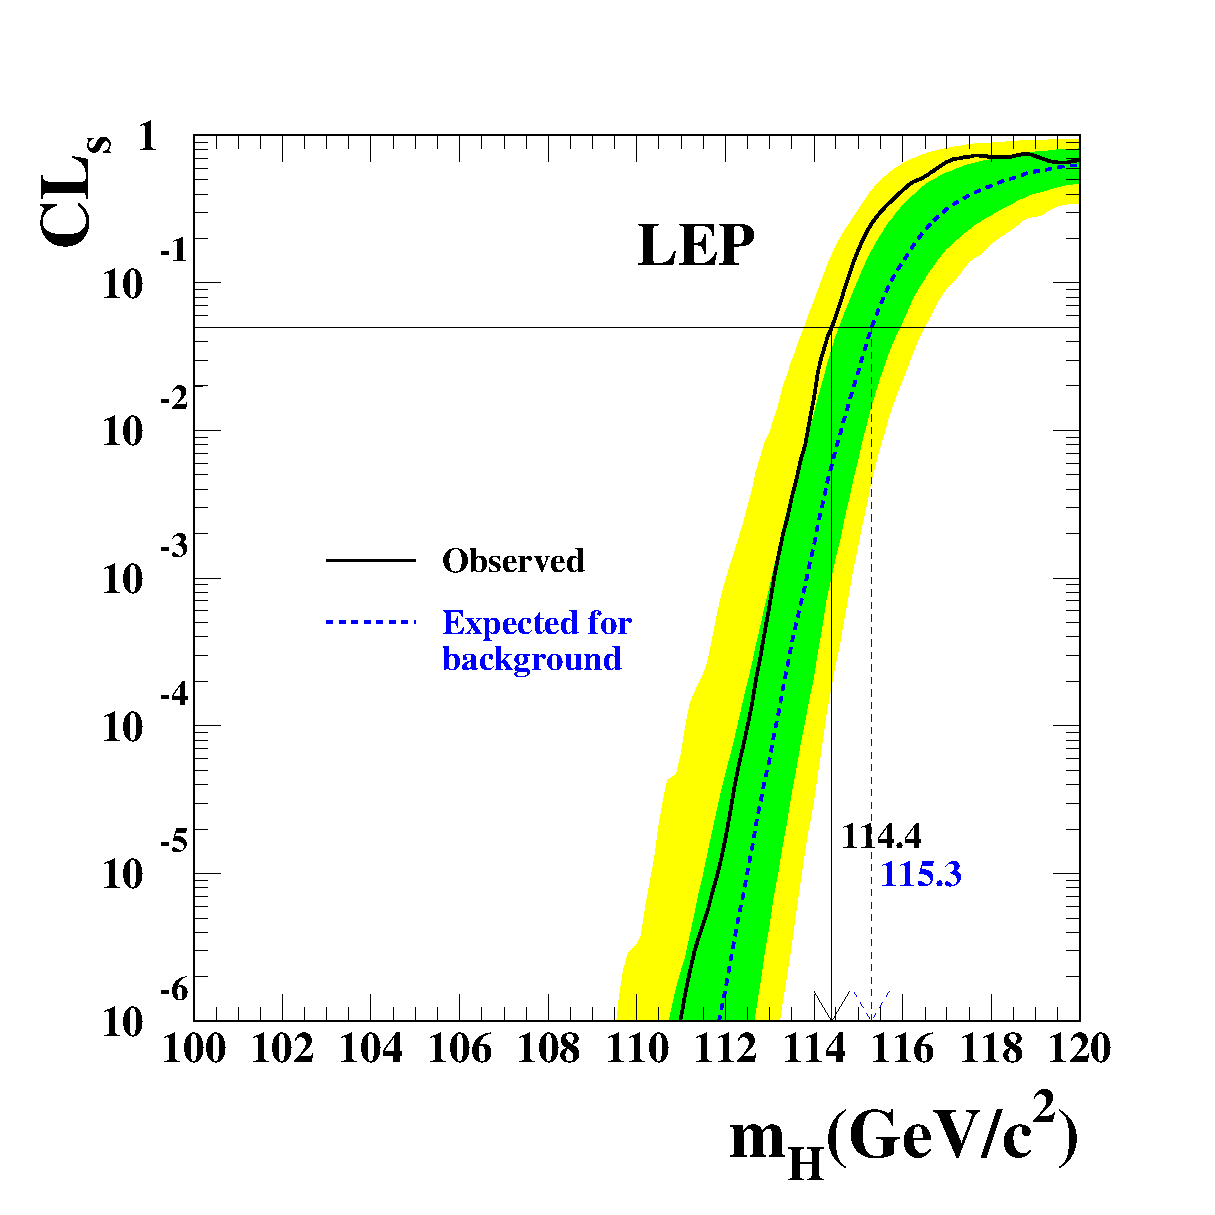
\includegraphics[width=0.7\textwidth]{StandardModel/fig9.eps}
\caption{\small The ratio $CL_S=CL_{(S+B)}/CL_B$
 for the signal plus background hypothesis. Solid line: observation; dashed line:
median background expectation. The dark and light shaded bands around the median
expected line correspond to the 68\% and 95\% probability bands. The intersection of the horizontal line 
for 
$CL_S = 0.05$
 with the observed curve is used to define the 95\%
confidence level
lower bound on the mass of the Standard Model Higgs boson.~\cite{Barate:2003sz} }
\label{fig:adlocls}
\end{figure}

The Tevatron, at Fermilab, took data up to 2011 and was a proton-antiproton collider.  The center of mass energy of the Tevatron was 1.96 TeV.  The main mode of Higgs production studied at the Tevatron was $\Pp\Pap \rightarrow V\PH$ where $V$ is a vector boson $V\equiv \PWpm,\PZ$.  The decay products most studied is where the vector bosons decay into leptons.  The most promising Higgs decay was $\PH \rightarrow \PWp\PWm$ if the Higgs had a mass above 135 GeV.  The combination of the Tevatron results for the detectors, CDF, and D$\emptyset$ can be seen in Figure~\ref{fig:comboRatio}~\cite{CDFandD0:2011aa}. In addition to confirming part of the already excluded range from LEP, the range 149 to 182 GeV was excluded at the 95\% confidence level.

\begin{figure}[htb]
\centering
%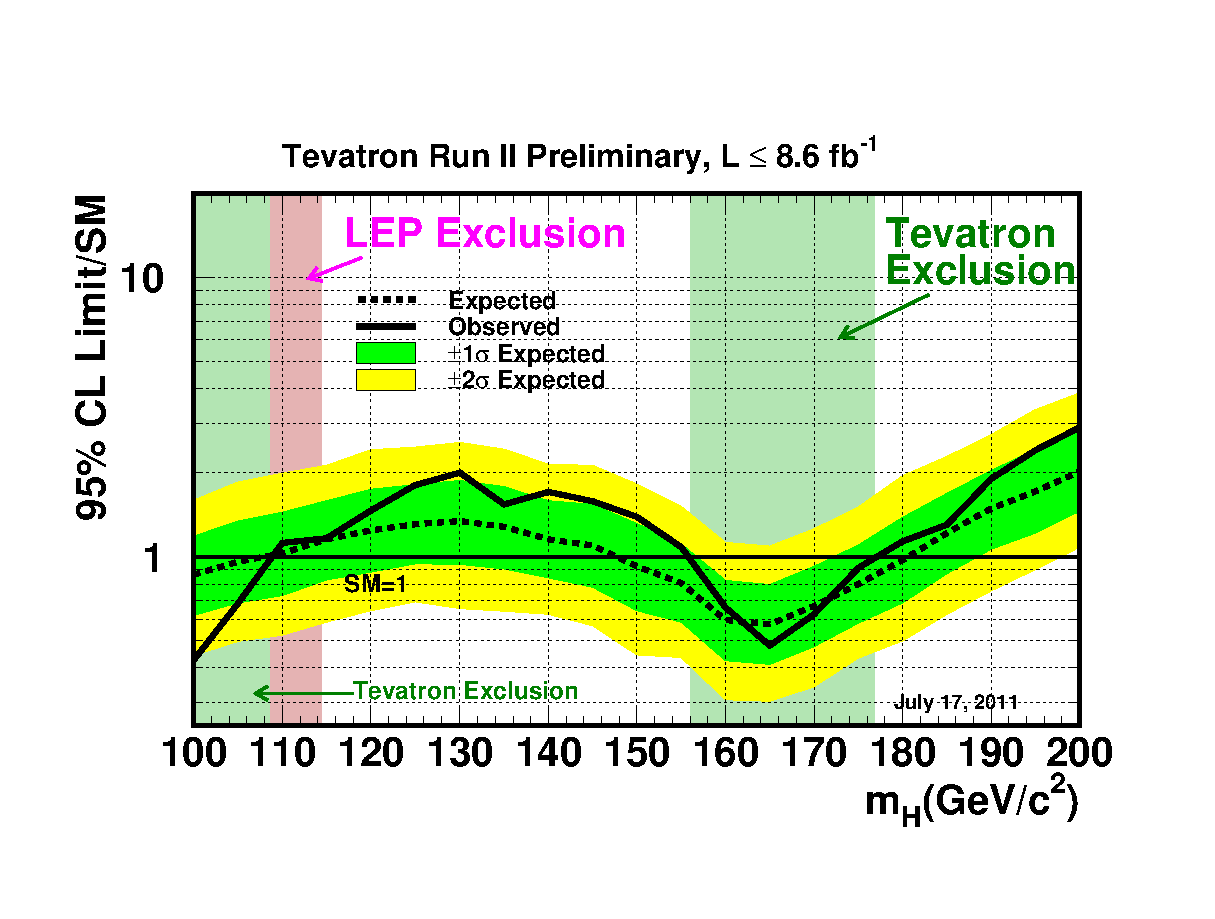
\includegraphics[width=0.8\textwidth]{StandardModel/tevbayeslimits17july2011.eps}
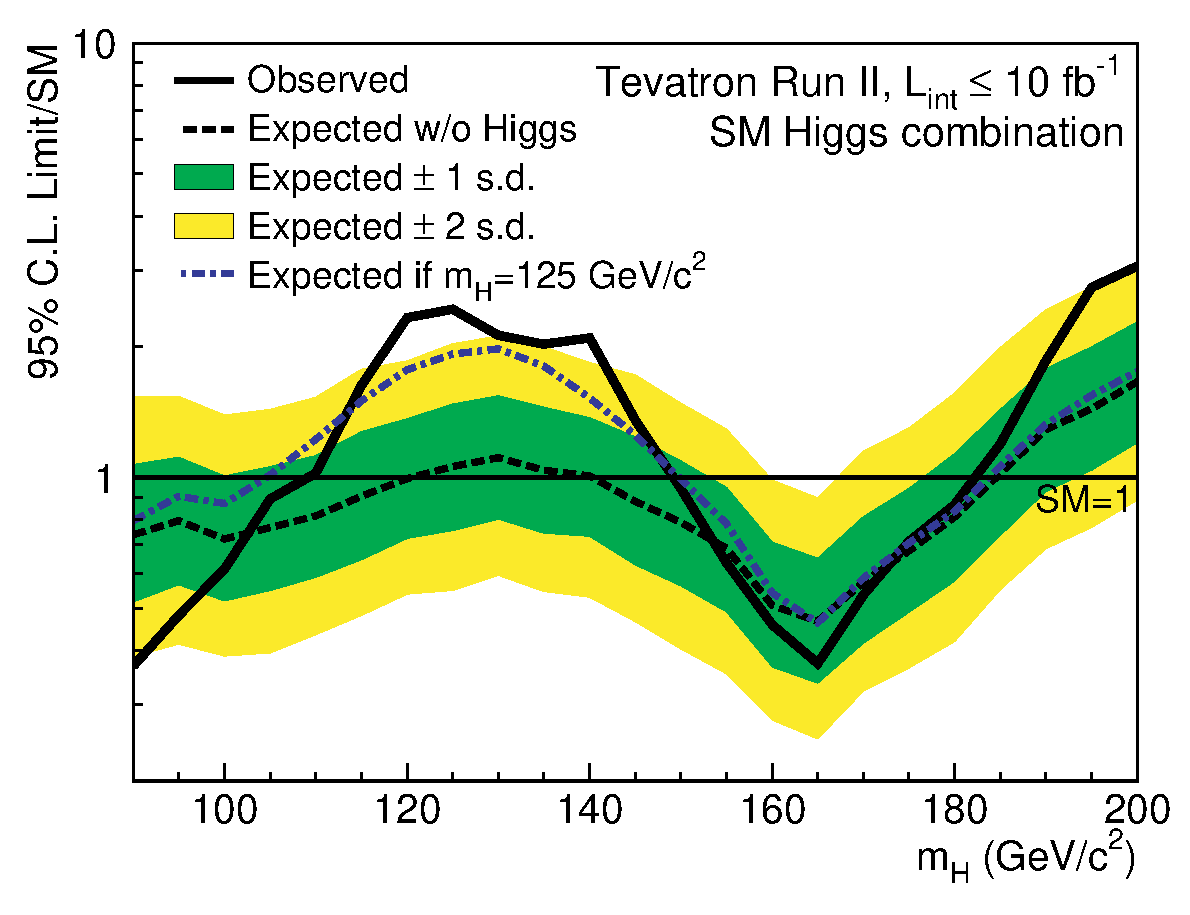
\includegraphics[width=0.8\textwidth]{StandardModel/tevsmlimits_feb2013.eps}
\caption{\small
Observed and median expected (for the background-only hypothesis) 95\% C.L. Bayesian upper production limits expressed as multiples of the SM cross section as a function of Higgs boson mass for the combined CDF and D0 searches in all decay modes. The dark and light shaded bands indicate, respectively, the 1 and 2 standard deviations probability regions in which the limits are expected to fluctuate in the absence of signal. The blue short dashed line shows median expected limits assuming the SM Higgs boson is present at m$_H$ = 125 GeV.~\cite{CDFandD0:2011aa}
%Also shown are the  expected upper limits obtained for
%all combined CDF channels, and for  all combined D0 channels.
}
\label{fig:comboRatio}
\end{figure}


Through fitting precision electroweak measurements, indirect measurements of the Higgs boson mass can be derived. Of particular usefulness is the changes in the vacuum polarization of the $\PZ$ and $\PWpm$ bosons through loop corrections. Figure~\ref{fig:indirect_greenband}~\cite{Flacher:2008zq} shows the $\Delta\chi^2$ variation of best fit to the combined data of LEP, Tevatron, and the Stanford Linear Accelerator (SLAC) accelerators, both with the pure indirect searches, and the combined direct and indirect searches.  While the lower Higgs masses are favored, even the high mass ranges were not completely ruled out.

\begin{figure}[htb]
\centering
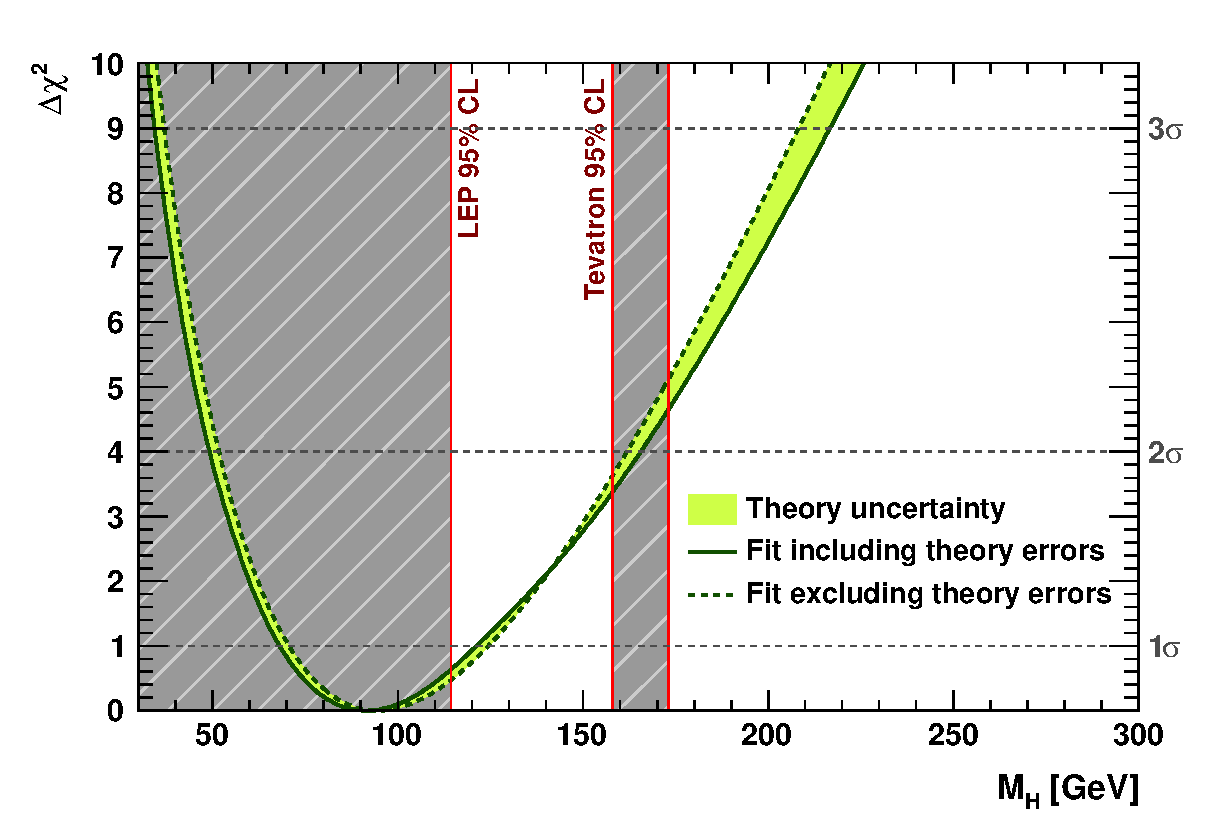
\includegraphics[width=0.7\textwidth]{StandardModel/HiggsScan.eps}
\includegraphics[width=0.7\textwidth]{StandardModel/HiggsScanDirectSearches.eps}
%   \centerline{\epsfig{file=Figures_Para/HiggsScanDirectSearches.eps, scale=\defaultFigureScale}}
%  \vspace{ 0.3cm}
\caption{\small Indirect determination of the Higgs boson mass: 
            $\Delta\chi^2$ as a function of $M_H$ for the standard fit (top) and the 
            complete fit (bottom). The solid (dashed) lines give the results when 
            including (ignoring) theoretical errors.~\cite{Flacher:2008zq}
         }
\label{fig:indirect_greenband}
\end{figure}






%\begin{fmffile}{simple}
%  \begin{fmfgraph}(40,25)
%    % Note that the size is given in normal parentheses
%    % instead of curly brackets.
%    % Define external vertices from bottom to top
%    \fmfleft{i1,i2}
%    \fmfright{o1,o2}
%    \fmf{fermion}{i1,v1,o1}
%    \fmf{fermion}{i2,v2,o2}
%    \fmf{photon}{v1,v2}
%  \end{fmfgraph}
%\end{fmffile}
%
%	    \begin{fmffile}{gluon}
%	        \begin{fmfgraph}(40,25)
%	            \fmfleft{in}
%	            \fmfright{out}
%	            \fmf{curly}{in,out}
%	        \end{fmfgraph}
%	    \end{fmffile}



%Within the framework of relativistic quantum field theory the Standard Model is a description of the microscopic world in terms of interaction particles and fields.\cite{Ryder1996} It can be divided into two parts: quantum chromodynamics (QCD) and quantum electrodynamics (QED). This allows us to write the Lagrangian as the summation of two separate parts:
%\begin{equation}
%\mathcal{L}_{SM} = \mathcal{L}_{QED} + \mathcal{L}_{QCD}
%\label{eq:sum_lagrandian}
%\end{equation}
%In QED the unphysical infinite contributions can always be eliminated.  This means that the theory is renormalizable. The Standard Model is renormalizable and also is compatible with special relativity. In 1960 Sheldon Glashow combined electromagnetism and weak interactions together to form the basis of the electroweak theory of interactions.\cite{Glashow1961} 



%\section{The Higgs Mechanism}

%If a doublet of scalar fields is introduced then its self-interactions provide spontaneous symmetry breaking and give masses to the gauge and fermion fields. This addition to the Lagrangian is $\mathcal{L}_{\Phi}$ and $\mathcal{L}_{\Phi}^F$ which are described in Equation ~\ref{eq:lagrangian_scalar}. It also introduces the Higgs boson, a new neutral scalar particle. 
%\begin{equation} \mathcal{L}_{\Phi} = |D_{\mu}\Phi|^2 - V(|\Phi|^2) \label{eq:lagrangian_scalar}\end{equation}
%For the scalar potential V the most general form that is renormalizable is Equation ~\ref{eq:potential_V}.
%\begin{equation} V = \mu^2|\Phi|^2 + \lambda|\Phi|^4 \label{eq:potential_V}\end{equation}

%From this the Higgs mechanism allows the vacuum to emit or absorb a Higgs boson. The coupling of the W and Z bosons to the Higgs field effectively gives them mass, while because the photon and gluon cannot couple to it they remain mass-less.

\section{The LHC Higgs Boson Search}

\subsection{LHC Higgs Production}

The Large Hadron Collider (LHC) at Cern is a proton-proton (pp) collider.  It had a center of mass energy of 7 TeV in 2010-2011 which increased to 8 TeV in 2012.  It reached an instantaneous luminosity of approximately $5 \times 10^{33} cm^{-2}s^{-1}$ ~\cite{1748-0221-3-08-S08001} in 2012.  There are four Higgs production processes at the LHC which are listed in Table~\ref{tab:lhc_higgs_production} in order of decreasing cross section.  The corresponding Feynman diagrams are in Figure~\ref{fig:Higgs_Feynman_diag} ~\cite{Egede_Feynman_Higgs}.  The cross sections for each of these processes at both $\sqrt{s}$ = 7 TeV and $\sqrt{s} =$ 8 TeV can be seen in Figure~\ref{fig:LHC_higgs_production} ~\cite{LHC_Higgs_Gallery}. It is important to note that changing from 7 Tev to 8 TeV increased the inclusive Higgs boson production cross-section at $m_H$ = 125 GeV by about 25\%. 

Gluon gluon fusion is the dominant Higgs production process at the LHC center of mass energies. Vector boson fusion (VBF) is the second highest production cross section with about one order of magnitude less than gluon gluon fusion.  In the very high mass region the processes become more comparable.  Despite this lower cross section, VBF is extremely powerful because of the two spectator jets that have a large invariant mass.  This signature allows fantastic background discrimination which increases the signal to background ratio greatly. The following analysis mainly deals with these two processes. 



\begin{table}[htb]
\caption{%
  \small Higgs production processes at the LHC. %
}
\begin{center}
\begin{tabular}{ | c | c | }
\hline
gluon gluon fusion & $\Pg\Pg \rightarrow \PH$ \\ \hline
vector boson fusion & $\Pq\Pq \rightarrow \PH\Pq\Pq$ \\ \hline
associated production & $\Pq\Paq \rightarrow \PW\PH,\PZ\PH$ \\ \hline
associated production with top quarks & $gg,\Pq\Paq \rightarrow \Pqt\Paqt\PH$ \\ \hline
\end{tabular}
\end{center}
\label{tab:lhc_higgs_production}
\end{table}

\begin{figure}[htb]
\centering
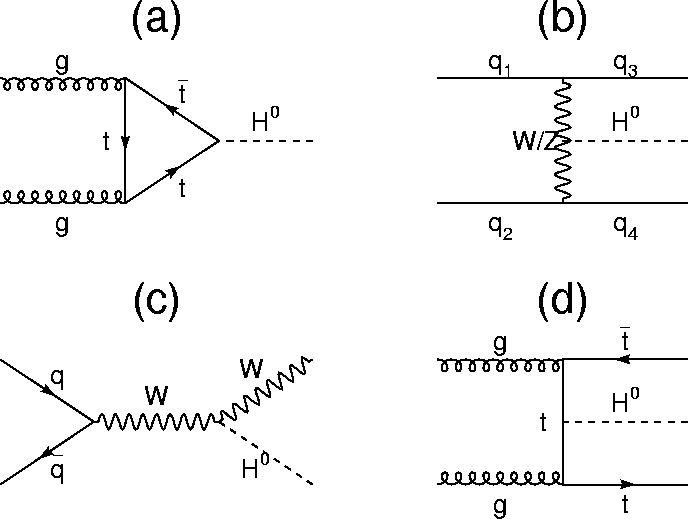
\includegraphics[width=0.7\textwidth]{StandardModel/feynman_higgs_production.jpg}
%   \centerline{\epsfig{file=Figures_Para/HiggsScanDirectSearches.eps, scale=\defaultFigureScale}}
%  \vspace{ 0.3cm}
\caption{\small The most important processes for Higgs production at hadron colliders. Gluon fusion (a), vector boson fusion (b), Associative production with W (c) and an example of the diagrams having associative production with a top pair (d). ~\cite{Egede_Feynman_Higgs}
         }
\label{fig:Higgs_Feynman_diag}
\end{figure}


\begin{figure}[htb]
\centering
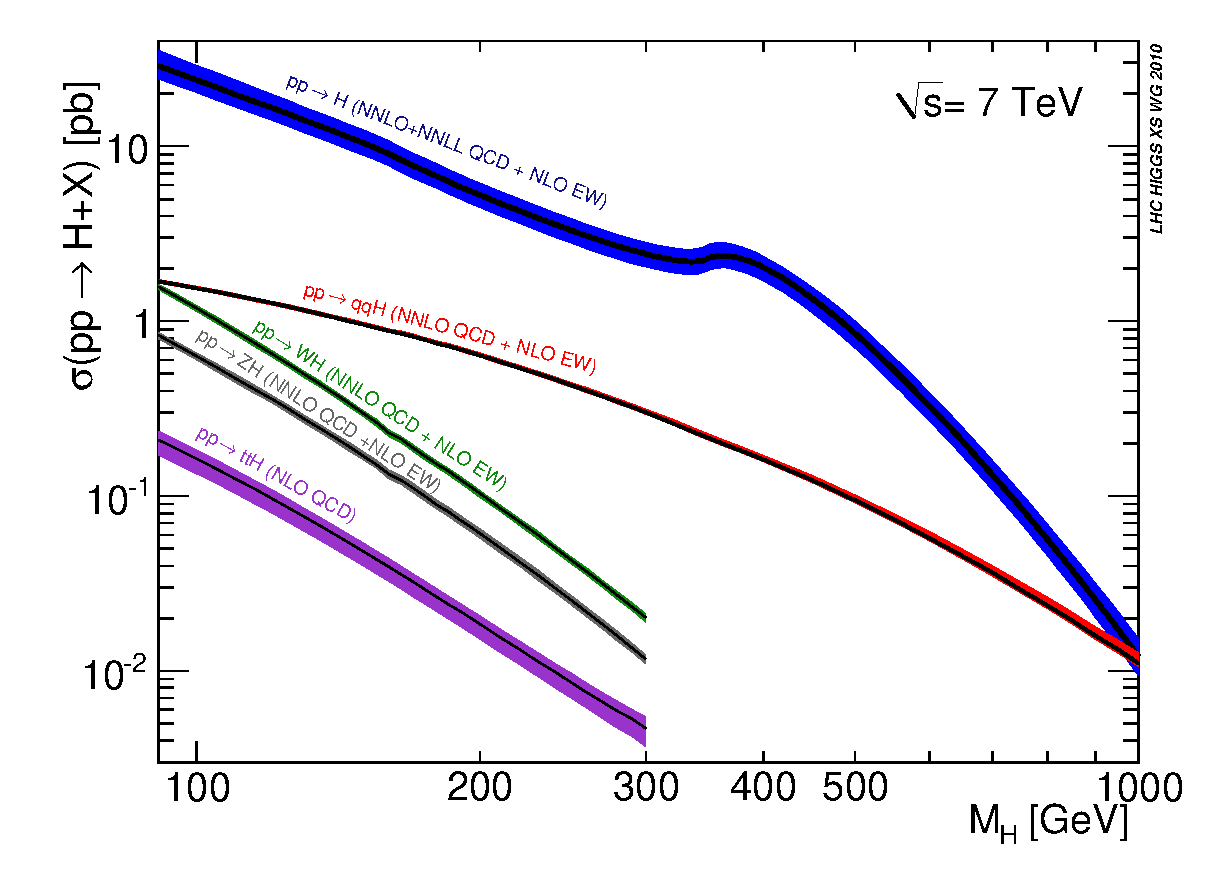
\includegraphics[width=0.7\textwidth]{StandardModel/Higgs_XS_7TeV.eps}
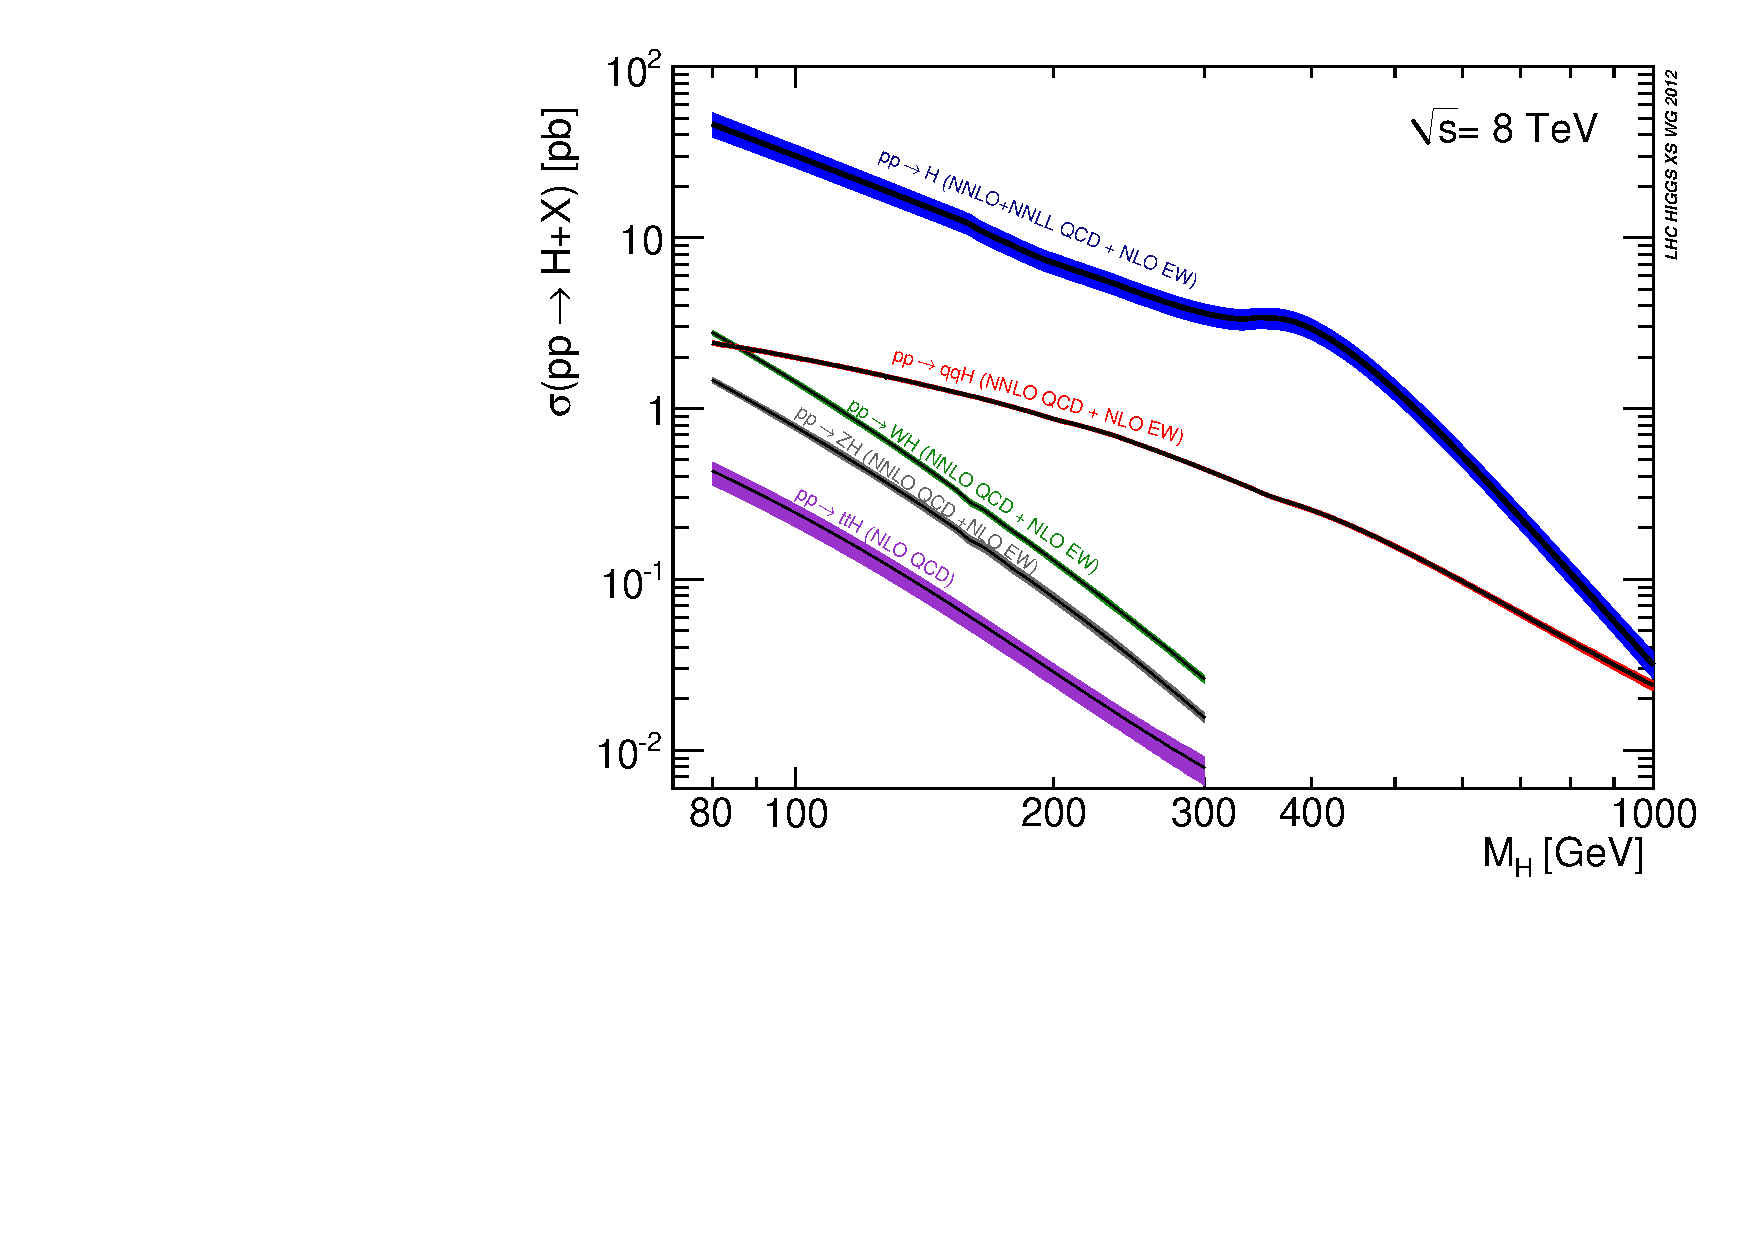
\includegraphics[width=0.7\textwidth]{StandardModel/Higgs_XS_8TeV_lx.pdf}
\caption{\small Standard Model Higgs boson production cross sections at $\sqrt{s}$ = 7, 8 TeV. Transition for VBF at MH=300 GeV at 8 TeV is due to change from ZWA to complex-pole-scheme.~\cite{LHC_Higgs_Gallery}
         }
\label{fig:LHC_higgs_production}
\end{figure}

\subsection{Higgs Decay}

The Higgs boson can decay into a variety of other particles.  The branching ratios of this decay are shown in Figure~\ref{fig:Higgs_decay}~\cite{LHC_Higgs_Gallery}.  From these images we can see that in the low mass region the most important decays are the fermions with $\PH \rightarrow \Pqb\Paqb$.  This is most important because the b quark is the heaviest fermion available.  As soon as it is possible to create vector boson pairs they begin to dominate the branching fraction.  Also in the high mass region (above 350 GeV) $\Pqt\Paqt$ pairs are created.  An important thing to note is that the best Higgs decay channels are not only those with large branching ratios, but also those in which a good signal to background ratio can be achieved. There are three Higgs mass regions that have different properties in this respect.


\begin{figure}[htb]
\centering
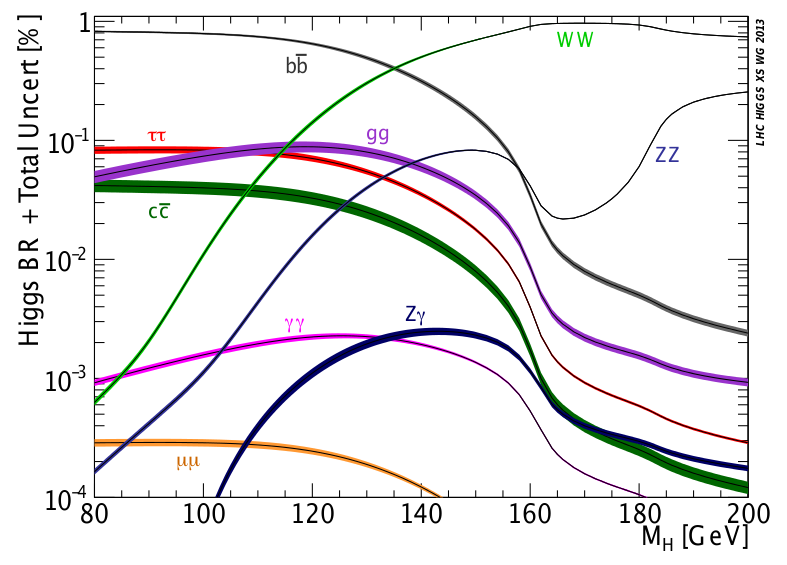
\includegraphics[width=0.8\textwidth]{StandardModel/Higgs_BR_LM_RECT.png} 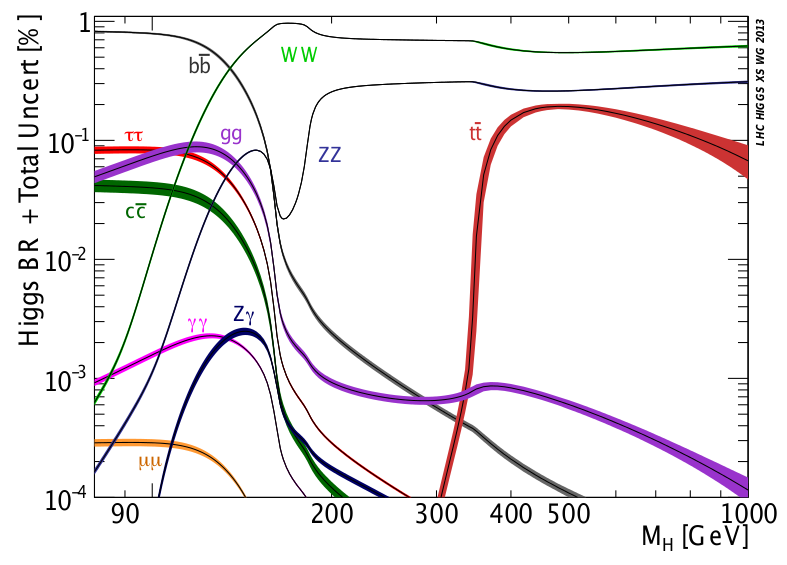
\includegraphics[width=0.8\textwidth]{StandardModel/Higgs_BR_RECT.png}
\caption{\small Standard Model Higgs boson decay branching ratios for two different $m_H$ ranges. ~\cite{LHC_Higgs_Gallery}
         }
\label{fig:Higgs_decay}
\end{figure}


In the low mass region ($m_H < 120$ GeV), even though the dominant decay is $\PH \rightarrow \Pqb\Paqb$, the bb di-jet backgrounds make this channel extremely difficult to use.  The most promising channel is the $\PH \rightarrow \Pgg\Pgg$.  The reason this channel works well is because the signature is so clear and there are only the $\Pq\Paq \rightarrow \Pgg\Pgg$ and the $\PZ \rightarrow \Pep\Pem$ backgrounds.  In the mid mass region (120 GeV $< m_H <$ 135 GeV) $\PH \rightarrow \Pgg\Pgg$ is still available but also $\PH \rightarrow \PW\PW^*, \PZ\PZ^*, \PZ\Pgg$. The real winner of these is the $\PH \rightarrow \PZ\PZ^* \rightarrow 4\Pl$ because even though it has a lower branching ratio than $\PW\PW^*$, it has a very clear decay signature and is able to fully reconstruct the Higgs mass.  In the high mass region ($m_H >$ 135 GeV) both the $\PW\PW$ and $\PZ\PZ$ channels begin to dominate.  Despite the lower branching ratio of the  $H \rightarrow \PZ\PZ$ decay, the clean signature allows fantastic background rejection.


\subsection{H $\rightarrow$ ZZ $\rightarrow l^{+}l^{-} \Pq \Paq$ Channel}
In the high mass region for a Higgs boson discovery the predominant Higgs decay is to vector boson pairs, H $\rightarrow$ WW and H $\rightarrow$ ZZ.  The signatures from the fully leptonic decay modes for these two processes are easily reconstructible and can be distinguished from the background processes.  The fully leptonic decay modes are H $\rightarrow$ WW $\rightarrow$ $l^{+} \Pgn l^{-} \Pagn$ and H $\rightarrow$ ZZ $\rightarrow$ $l^{+}l^{-}l^{+}l^{-}$. The H $\rightarrow$ ZZ $\rightarrow$ $l^{+}l^{-}l^{+}l^{-}$ channel is particularly interesting because the decay chain can be fully reconstructed with a narrow invariant mass peak and almost no Standard Model background. The rate of decay of Z $\rightarrow$ $l^{+}l^{-}$ is only 3.37\% \cite{PDG2012} so for $ l = e,\Pgm$ there is only a 0.45\% chance of ZZ $\rightarrow$ $l^{+}l^{-}l^{+}l^{-}$.

The largest Z branching ratio is 69.9\% for Z $\rightarrow \Pq \Paq$ \cite{PDG2012}. Furthermore, ZZ $\rightarrow \Pq \Paq \Pq \Paq$ has a decay probability of just under 50\%. The problem is that while this maximizes the branching ratio, this final state is indistinguishable from Standard Model background processes, like QCD.

The semi-leptonic final state in H $\rightarrow$ ZZ $\rightarrow l^{+}l^{-} \Pq \Paq$ produces a number of benefits over the previous two decay channels.  The branching ratio of ZZ $\rightarrow l^{+}l^{-} \Pq \Paq$ is 9.4\%, or more than 20 times as large as ZZ $\rightarrow$ $l^{+}l^{-}l^{+}l^{-}$. This can be seen in the plots of Higgs decay cross section multiplied by the final state branching ratio for both 7 TeV and 8 TeV in Figure~\ref{fig:XSBR}~\cite{LHC_Higgs_Gallery}. In comparison to ZZ $\rightarrow \Pq \Paq \Pq \Paq$ the leptonic decay of one of the Z bosons significantly reduces the Standard Model background in the final state.

\begin{figure}[htb]
\centering
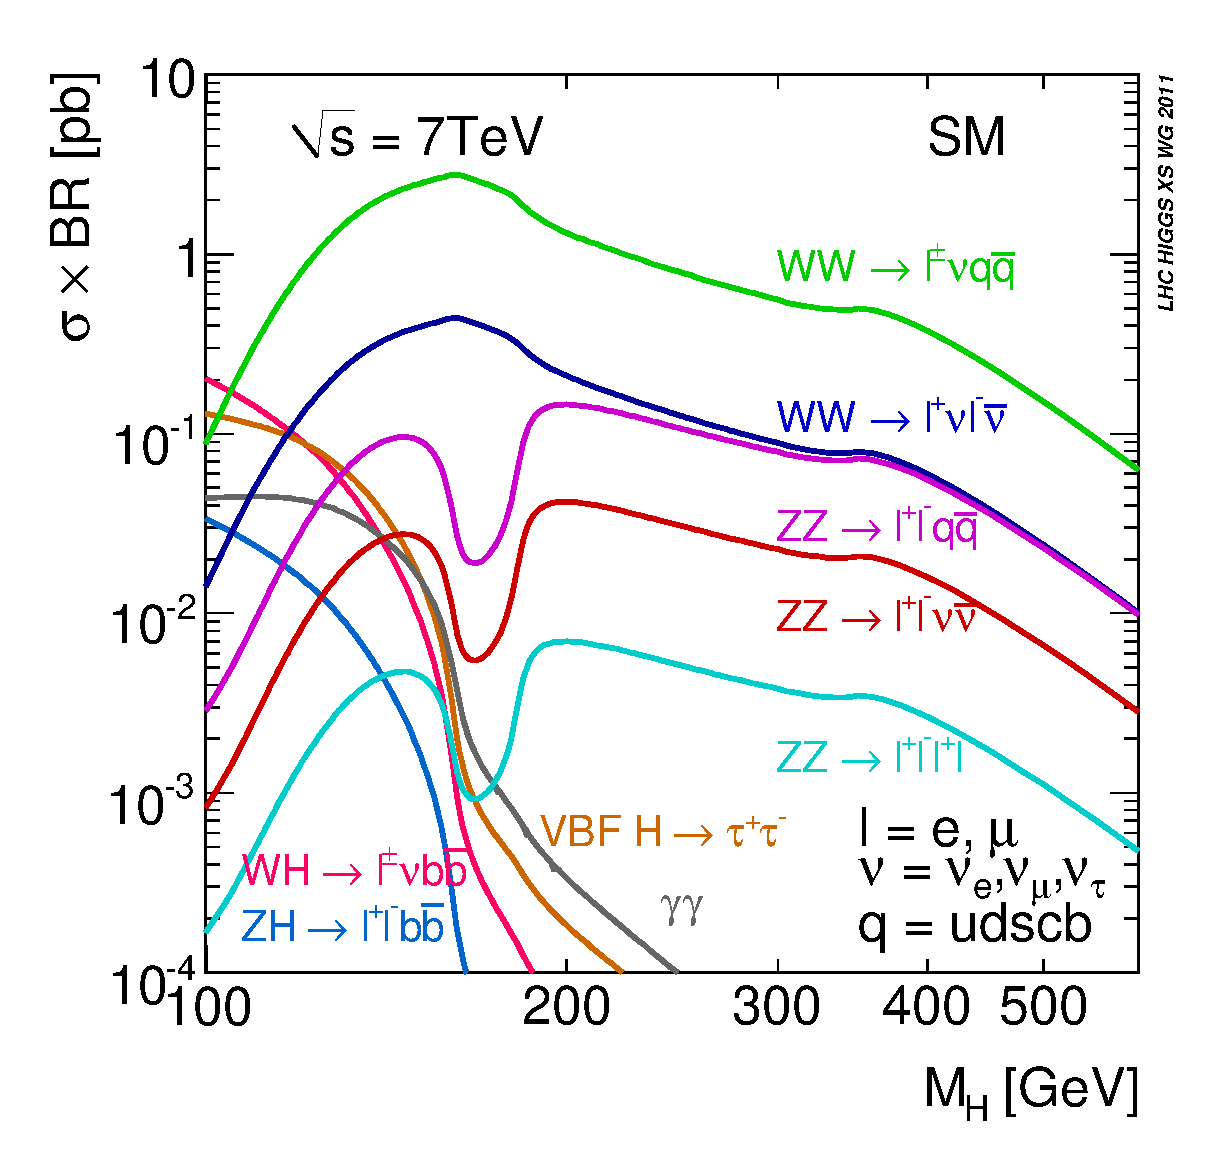
\includegraphics[width=0.7\textwidth]{StandardModel/XSBR_7TeV_SM.eps} 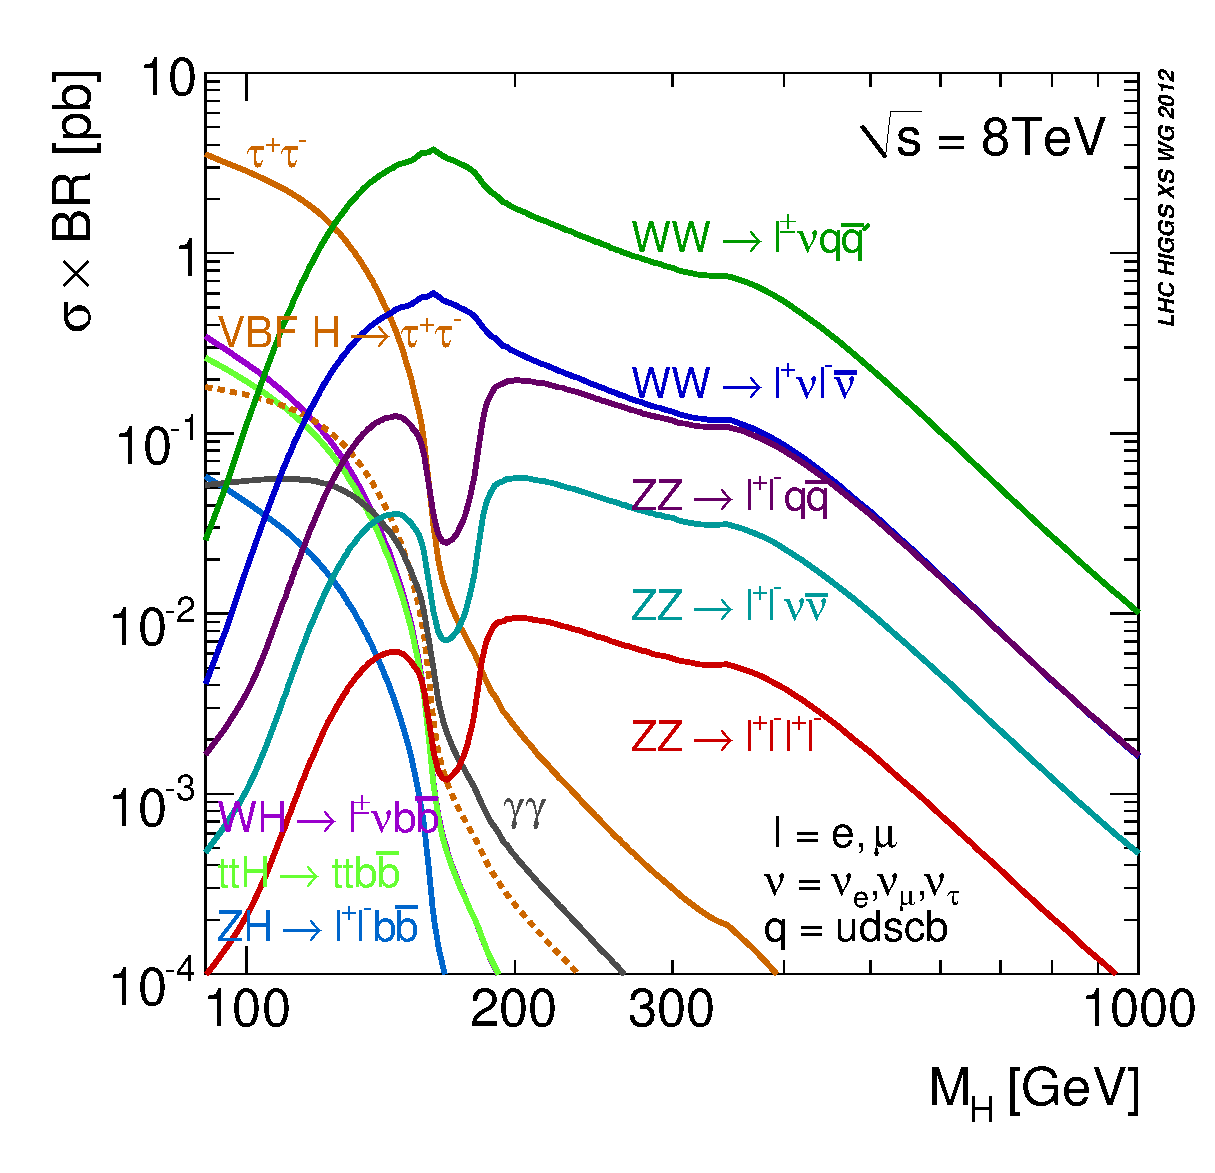
\includegraphics[width=0.7\textwidth]{StandardModel/XSBR_8TeV_SM_HM.eps}
\caption{\small Standard Model Higgs boson production cross section times branching ratio at $\sqrt{s}$ = 7 TeV and 8 TeV. ~\cite{LHC_Higgs_Gallery}
         }
\label{fig:XSBR}
\end{figure}



Some of the difficulties in this channel compared to the fully leptonic decay are increased difficulty in event selection, the final reconstruction efficiency is approximately half of the fully leptonic final state, the backgrounds are significantly higher and dominated by Z+jets final states, and the resolution is worse.  Despite these difficulties, this channel has improved sensitivity over the fully leptonic final state at high masses because of the higher branching ratio that the semi-leptonic final state enjoys, and at high masses the Z+jets background is not as significant.



\subsubsection{$l^{+}l^{-} \Pq \Paq$ Background Contamination}

The background processes for this channel are processes which have a pair of opposite signed leptons with high transverse momentum that are associated with two jets.  The main backgrounds are listed in Table~\ref{tab:background_2l2q}.

\begin{table}[htb]
\caption{%
  The main Standard Model background processes for the H $\rightarrow$ ZZ $\rightarrow l^{+}l^{-} \Pq \Paq$ channel and their cross sections at 8 TeV.
}
\begin{center}
  \begin{tabular}{ | c | c |} \hline
    Background Process & Cross Section [pb] at 8 TeV\\ \hline \hline
    $\PZ + jets$ & 3503.71 \\ \hline
    $\Pqt \Paqt$ & 225.197\\ \hline
  %  $\Pqt \PWm$  & \\ \hline
  %  $\Paqt \PWp$ & \\ \hline
    $\PZ \PZ$    & 17.654 \\ \hline
    $\PW \PZ$    & 22.88 \\ \hline
    $\PW \PW$    & 57.1097\\ \hline
  \end{tabular}
\end{center}
\label{tab:background_2l2q}
\end{table}

The dominant background in the  $\PH \rightarrow \PZ\PZ \rightarrow l^{+}l^{-} \Pq \Paq$ analysis is the Z+jets background, or more specifically, the inclusive $\PZ$ production with QCD jets.  The cross section of Z production at the LHC is more than 10$^{4}$ larger than the Higgs signal.

Events containing top quarks are another significant source of background.  There are two top processes that result in the same final state as the signal we are studying.  They include $\Pqt \Paqt$ pair production and top quark associated production with a $\PW$ boson.
\begin{center}
  \begin{tabular}{ c }
    $\Pqt \Paqt  \rightarrow (\PWp \rightarrow \Plp\Pgn)\Pqb (\PWm \rightarrow \Plm\Pagn)\Paqb           $
  \end{tabular}
\end{center}
